\documentclass{article}
\usepackage{graphicx} % Required for inserting images

\title{DevOps24-groupK\\
\large Course Code: BSDSESM1KU}
\author{GitGurus}
\date{Spring 2024}

% \usepackage{graphicx} % Required for inserting images
% \usepackage{amsmath}
% \usepackage{hyperref}
\usepackage{listings}
\lstset
{
    basicstyle=\footnotesize,
    numbers=left,
    stepnumber=1,
    showstringspaces=false,
    tabsize=1,
    breaklines=true,
    breakatwhitespace=false,
}

\usepackage[utf8]{inputenc}
\usepackage[T1]{fontenc}
\usepackage[english]{babel}
\usepackage{minted}
% \usepackage[a4paper, bottom=3cm, top=3cm, left=2.5cm, right=2.5cm]{geometry}
\usepackage[linewidth=1pt]{mdframed}
\usepackage{ebproof}
\usepackage{amsmath}
% \usepackage{fourier}
\usepackage{booktabs}
% \usepackage{inconsolata}
\usepackage{float}
\usepackage{lastpage}
\usepackage{graphicx}
\usepackage{titling}
\usepackage{fancyhdr}
\usepackage[dvipsnames]{xcolor}
\usepackage[hidelinks]{hyperref}

\renewcommand{\baselinestretch}{1.2} % Line spacing
% \setlength{\parindent}{0em} % Paragraph indent
% \setlength{\parskip}{0.75em} % Paragraph vertical spacing

% \colorlet{LightGray}{Gray!7!}

% % global minted styles
% \setminted{bgcolor=LightGray, breaklines, frame=single, linenos, fontsize=\small, numbersep=8pt}

% % minted remove red squares around "erroneus" code
% \AtBeginEnvironment{minted}{%
%   \renewcommand{\fcolorbox}[4][]{#4}}

% % minted line number style
% \renewcommand{\theFancyVerbLine}{{\scriptsize \arabic{FancyVerbLine}}}
\begin{document}

\maketitle

\begin{table}[H]
    \centering
    \begin{tabular}{r|l}
    Andreas Guldborg Hansen & aguh@itu \\
    Andreas Severin Hauch Trøstrup & atro@itu.dk \\
    Frederik Petersen & frepe@itu.dk \\
    Mads Aqqalu Roager & mroa@itu.dk \\
    Silke Holme Bonnen & ssbo@itu.dk
    \end{tabular}
\end{table}

\newpage
\tableofcontents

\newpage


\section{Systems' perspective}
\subsection{Design and architecture}
An overview of the architecture of our MiniTwit application can be found in figure \ref{fig:architecture}. 
The entire system runs on DigitalOcean, with the exception of our monitoring and logging that runs on New Relic.
In DigitalOcean, we have 3 primary nodes running. A swarm manager, and two workers. These 3 nodes are a part of a docker swarm network that runs the minitwit web app and minitwit simulator API containers as docker services.
The workers and manager also run a New Relic agent that collects logs and system monitoring information. This information is then sent to New Relic.
The manager node runs a Nginx reverse proxy, that handles https encryption, and load balancing between the workers.
Lastly, in DigitalOcean we also have a managed database running, that acts as the database for the application.
What the diagram below does not show is that the swarm manager also has a container running the web app and the simulator API. The reason why this is not shown on the diagram is because the Nginx reverse proxy has been set to only forward requests to worker 1 and 2. 
That means that the web app and the simulator api in the swarm manager will never be used. 


\begin{figure}[H]
    \centering
    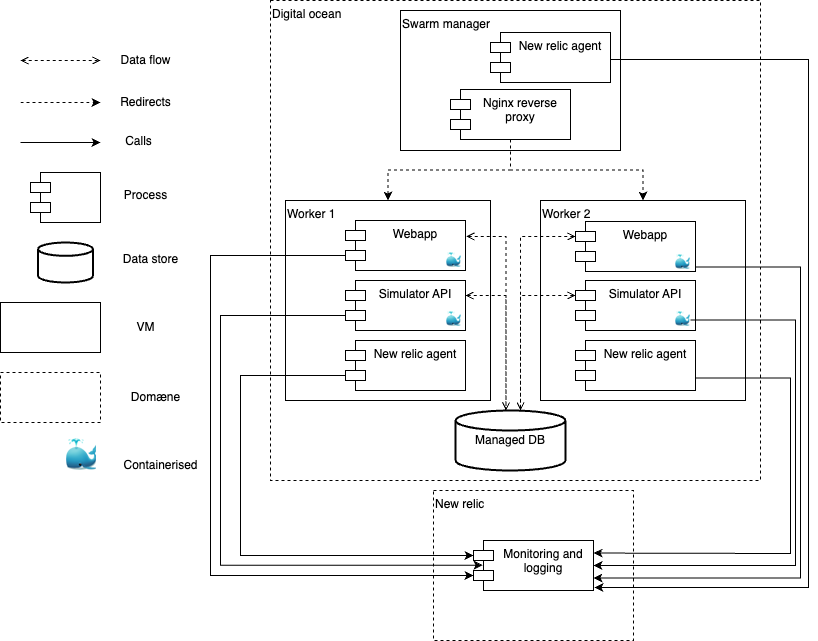
\includegraphics[width=\textwidth]{images/devops-overview.png}
    \caption{The figure shows a diagram of the architecture of minitwit}
    \label{fig:architecture}
\end{figure}

\subsection{Dependencies}
Our application has numerous dependencies, so we have decided to only describe the dependencies that are critical to our application in production. That is, if there is a problem with one of these dependencies, e.g. a dependency has a open security problem, we have a problem. 

In the dependency graph, available in Figure \ref{fig:dep-prod}, only the direct dependencies in production is shown, with one exception -- PostgreSQL is shown as a dependency to DigitalOcean. We decided that it was important to show this dependency as it is a critical dependency for our application.
Besides from this, we do not show what our dependencies depend on and we do not show the development dependencies. The most important development dependencies can be seen in appendix \ref{appendix: dev-dependecies}.

\begin{figure}[H]
    \centering
    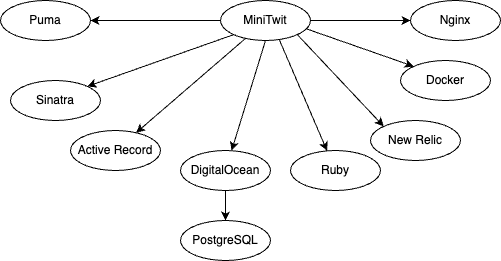
\includegraphics[width=0.8\textwidth]{images/dependency-graph-prod.png}
    \caption{Production dependency graph.}
    \label{fig:dep-prod}
\end{figure}

Puma is the webserver used for deploying our Ruby application. 
To develop our web application we use Sinatra, which is a web application library for Ruby. 
The Object-Relational Mapping (ORM) library Active Record is used to simplify interactions with the database. This enables us to avoid having SQL statements in our code which keeps the code more clean and leaves security threats related to database interactions to be handled by Active Record. 

DigitialOcean is the only critical dependency for keeping the application running. This means that it is the only dependency that would make our application crash right away if it stopped working. DigitalOcean holds our 3 VM's and the database. Furthermore we also depend on DigitalOceans DNS servers. 
PostgreSQL is the database management system used for the database. It is hosted as a managed database on Digital Ocean. Thus, Digital Ocean depends on PostgreSQL in our system, depicted in Figure \ref{fig:dep-prod}.

Ruby is the programming language used to develop the minitwit application.
New Relic is used for monitoring and logging of the system. It is a push-based monitoring system, and thus each of our VMs runs a New Relic agent that collects and sends logs and monitoring data to New Relic.

Docker is used for containerization of our application, such that it runs as long as our VM has docker installed. The application is run with Docker Swarm, which ensures that the application runs across several machines, and makes load-balancing possible. It also makes it possible to make updates to the application with minimal downtime.

Nginx, is a reverse proxy and load balancer we use to expose the minitwit web application. It takes http requests from minitwit.tech, and load balances the request to a worker in the docker swarm. It then takes the reply from the worker and replies the client through https://minitwit.tech with a generated certificate, and thus achieves both load balancing and security in the form of SSL encryption.

\subsection{Interactions of subsystems}

The interactions between MiniTwit's subsystems is explained through two sequence diagrams of a user interacting with MiniTwit's web app and the API. 
\\\\
Diagram \ref{fig:sequence} starts with a user trying to access minitwit.tech through a browser. The first part of the diagram shows how the DNS protocol is utilized in order to get the IP address of the server. The second part shows how the Nginx reverse proxy, located inside the swarm manager, forwards the HTTP request to worker 1 or 2. Inside the worker the web application is running in a container. When the application gets the request it queries the database to get the latest messages. While the application handles the request a new relic ruby agent monitors the request and forwards the information to New Relic. Finally a response gets propagated all the way back to the browser.
\\\\
Similarly, the diagram for the simulator API available in Figure \ref{fig:sequence_api} starts with the actor sending a HTTP GET request to api.minitwit.tech. In this diagram we omitted the DNS protocol as it is shown in detail in figure \ref{fig:sequence}. The Nginx reverse proxy forwards the request to worker 1 or 2, that then checks if the request originated from the simulator by checking if the header of the request was set correctly. If it was, it queries the database for the latest \textit{no} messages, where \textit{no} denotes a parameter set to specify how many messages should be returned. While the application handles the request a new relic ruby agent monitors the request and forwards the information to New Relic. Finally the response gets propagated all the way back to the actor.

\begin{figure}[H]
    \centering
    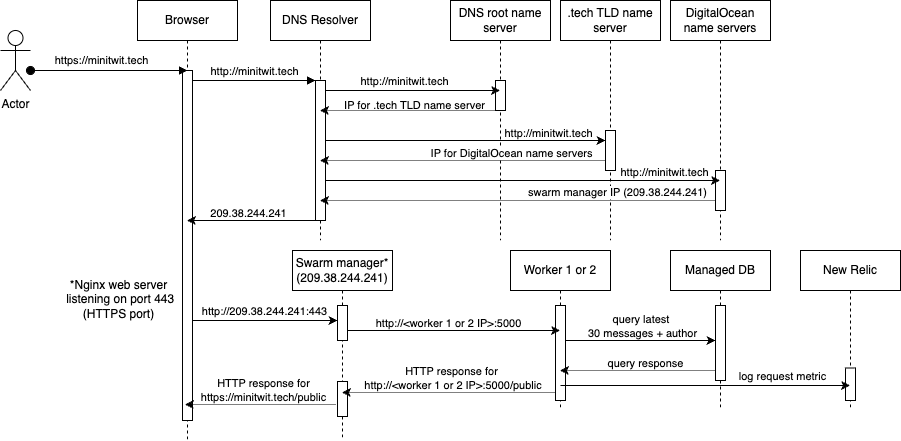
\includegraphics[width=\textwidth]{images/devops-sequence.png}
    \caption{The figure shows a sequence diagram describing a HTTP GET request to "minitwit.tech". }
    \label{fig:sequence}
\end{figure}


\begin{figure}[H]
    \centering
    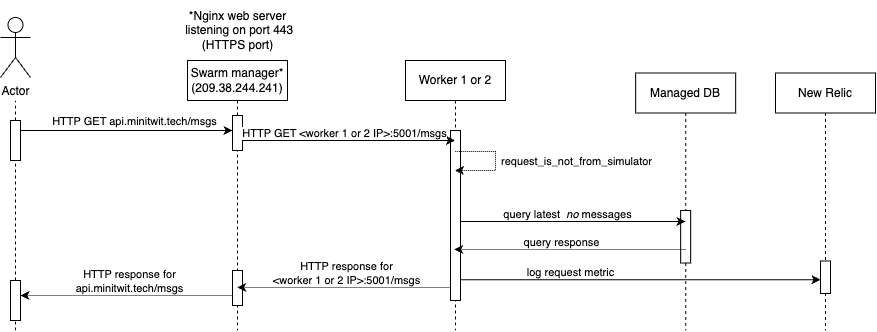
\includegraphics[width=\textwidth]{images/api-sequence.png}
    \caption{The figure shows a sequence diagram describing a HTTP GET request to "api.minitwit.tech/msgs". It is assumed that the \texttt{request\_is\_not\_from\_simulator} returns false. Otherwise it would return immediately with status code 403.}
    \label{fig:sequence_api}
\end{figure}


\subsection{Current state}
SonarCloud and CodeClimate has been used for static analysis and quality assessment. 
The quality gate status on SonarCloud is passed and there are no issues and no security hotspots detected. The duplication of code is 1.7\% which is below the 3\% limit. Code Climate maintainability rating is A, and there is one issue about a function being too long. 

To reduce noise in our static analysis the test files have been excluded from the static analysis to focus on the quality and maintainability in the application code as test files has different coding standards. An example of how 
the coding standards differ can be seen in the documentation for playwright, our used e2e testing tool. They state that it is okay to have some duplication in your tests especially if it keeps your test clearer and easier to read and maintain \cite{playwright_best_practices}. 


\section{Process' perspective}
The project was developed using GitHub for version control and project management, using the Issues feature to track development tasks.


\subsection{CI/CD chain}
Our CI/CD chain is built using GitHub Actions. We have implemented workflows to automate testing, release and deployment of our code. We also use third-party tools as steps, including Dependabot, SonarCloud and CodeClimate for static analysis.

\subsubsection{Automatic testing}
When a pull request is opened on GitHub, the \texttt{automatic-testing} workflow is triggered. This workflow builds a Docker image with the branch code, and runs it as an image using our \texttt{docker-compose} configuration. The workflow then runs the Python-based integration tests against this Docker container, and reports if any tests fail. 

\subsubsection{Deployment workflows}
We have two different deployment workflows that are somewhat similar but with different targets. The first is manually triggered only and deploys to a staging environment, used to test small features or changes. However, once we switched to a swarm setup, this environment was no longer used. In general, this works similar to the production deployment workflow, but targets the correct environment and tags the Docker image with the git commit's SHA-value instead.\\
The main deployment workflow runs on every push to the main branch, which checks out the code and logs in to \texttt{Docker Hub}. The workflow then builds the docker image, tagging it \texttt{latest} and pushes the image to Docker Hub, making it easy to pull and build this production-ready Docker image. The last action of the workflow is to establish an \texttt{ssh} connection to the swarm manager from which it runs our deploy script.\\
Once \texttt{deploy.sh} runs on the manager node, it sets the necessary environment variables in order to connect to the managed database, log to NewRelic and pull the correct image from Docker Hub before using \texttt{Docker Swarm's} command to execute a rolling deployment of the new Docker image. The \texttt{./remote\_files/docker-compose.yml} file is responsible for configuring the Docker swarm, such that there is a single replica for the frontend application whereas three replicas exists for the API that the simulator uses.\\

\subsubsection{Release workflow}
A simple workflow exists to ensure automatic releases are created on GitHub every time new code is added to the main branch. This workflow simply uses the two actions \texttt{actions/checkout@v4} and \texttt{actions/create-release@v1} to create a release with a version tag and release name based on the commit's SHA-value.

\subsubsection{Report workflows}
To ensure our report in our repository is always up to date, we utilise a built-in synchronization between Overleaf and GitHub. Once changes are made that a group member wish to save, one click from within Overleaf synchronizes the contents to a separate repository in our GitHub organisation, which triggers two Github Actions workflows:
\begin{enumerate}
    \item A workflow from within this report repository that notifies our main repository of any changes made to our report repository.
    \item A workflow from within the main repository that is called by the previously mentioned workflow, which triggers a git submodule update and commits it to the repository.
\end{enumerate}

\subsection{Monitoring \& Logging}
Both monitoring and logging of this project is done using New Relic. By installing the New Relic agent on our VMs, and the new relic gem in our ruby application we can link it to the web interface. This is done via a push-based monitoring configuration, as all VMs push their data directly to New Relic. 
\\From the interface we can monitor a lot of metrics, but most importantly:
\begin{itemize}
    \item Web transaction time by application layer (See Figure \ref{fig:transaction-times})
    \item Throughput for the application (Requests per minute) 
    \item The slowest transactions, by average response time.
    \item Error rate of transactions
\end{itemize}
Additionally we've set new relic up to send us alerts on slack, should the application suddenly have a significantly lower application throughput than usual, or if the error rate rises.
\begin{figure}[H]
    \centering
    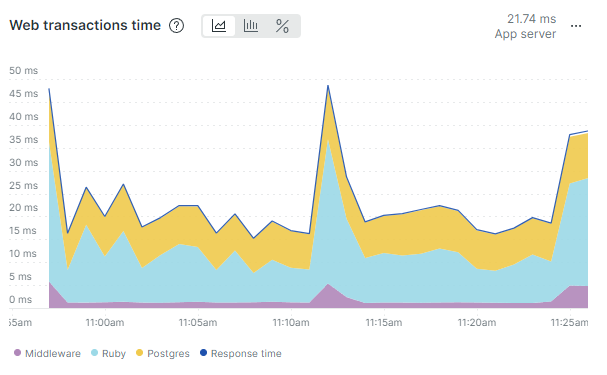
\includegraphics[width=\textwidth]{images/new-relic-transactions.png}
    \caption{The newrelic graph depicting web transaction times by application layer}
    \label{fig:transaction-times}
\end{figure}

Logs are aggregated automatically by the New Relic agent. The agent picks up log messages from any configured source. By default this includes the \texttt{syslog} and the docker log. In our case we aggregate \texttt{linux\_auth}, \texttt{linux\_syslog} and the \texttt{nginx} logs. The nginx logs shows all request made to the application on any of the VMs.

\subsection{Security}
The results of the security assessment yielded no obvious vulnerabilities, however we have had security in mind while making the application, especially in some aspects of the system. Firstly, we use an ORM to interact with the database in the application. This means that we do not have any explicit SQL statements in the code that can be exploited, and that ActiveRecord handles the security in terms of SQL injection prevention. Secondly, we have implemented HTTPS via. the Nginx reverse proxy. This means that all requests accessed at minitwit.tech are encrypted, and thus protects confidentiality. Lastly, we use a Docker Swarm to host the application, which makes the system more scalable and therefore easier to protect against a Distributed Denial-of-Service attack. We also use dependabot such that we will get notified when any dependency has an update, or has a security vulnerability.

\subsection{Scaling and upgrading}
% NB: Vi har skrevet lidt om det her i 2.1.2. Overvej om vi skal rykke noget derfra herned eller hvordan vi klarer det.
We have used start-first as our upgrade strategy. This corresponds to the blue-green upgrading strategy, where a new node starts before the old one stops. This enables us to perform updates without experiencing any downtime.


Horizontal scaling is used as our scaling strategy. This means that whenever an upscale is necessary another node will be added to the docker swarm as a replica of the system. We use Nginx as our load-balancer. This means that our swarm manager, which runs Nginx, becomes a single point of failure. It is always undesired to have single points of failures so if we had more time we would have liked to implement a redundant Load Balancer Setup, though this has not been investigated yet.


\subsection{Use of AI tools}
% \todo{In case you have used AI-assistants during your project briefly explain which system(s) you used during the project and reflect how it supported/hindered your process.}

In the beginning of the project, not all team members were familiar with the programming language Ruby. In order to get familiar, some of us had the Github Copilot extension enabled, allowing us to participate on a similar level as those who were more familiar with the language.
This helped the on the productivity but it might have hindered our learning, as you get the answers served on a plate instead of having to dig for it yourself.\\

In the review process, ChatGPT has been used as a tool to interpret changes made by other members, by prompting ChatGPT to help understand the effects and consequences of the changes. This has been a very helpful way to get complicated things explained quickly, and overall we believe that it has helped our learning experience. 

\section{Lessons learned perspective}
% \todo{Describe the biggest issues, how you solved them, and which are major lessons learned with regards to: evolution and refactoring,
% operation, and
% maintenance 
% of your ITU-MiniTwit systems. Link back to respective commit messages, issues, tickets, etc. to illustrate these. Also reflect and describe what was the "DevOps" style of your work. For example, what did you do differently to previous development projects and how did it work?}

% Paragraph: Evolving & Maintaining database (maybe)
% discuss what issues we had with migrating to new database. What did we learn from migrating
% we used NewRelic to identify missing indexes, to improve query speed (maintenance)
When we started out the project, the database was running as an SQLite database on the machine which also hosted our application. As the project progressed, we decided to migrate to a managed PostgreSQL database, hosted on DigitalOcean. Migrating to this new database was one of the bigger challenges in the project, as multiple problems in the process ended up causing us downtime.
The biggest issue was in how we transferred the data from SQLite to the new database. We created a simple migration script that read data from SQLite and inserted the corresponding data in PostgreSQL; however, we did not consider the scale of the data we were trying to handle.
As the migration script was trying to insert entire tables in a single statement, the script ended up crashing due to memory issues.
We addressed this issue by changing the migration script to perform the insertion in smaller batches -- this made the migration go smoothly, with no performance issues.
An important learning from this, is to always be careful when handling large amounts of data, as you might otherwise be inadvertently performing a Denial-of-Service against yourself, or worse, a third-party that might block further requests.

Another important learning was in how we identified and fixed issues with scaling our database. As the project went on, our database tables grew, and we started seeing noticeable performance issues on multiple endpoints. Here, our New Relic Application Monitoring proved to be essential in locating and fixing what turned out to be blatant performance issues. Looking at our response time metrics, we saw that one endpoint in particular was getting increasingly slower as our database grew larger. By looking at the query plan on New Relic we noticed the \texttt{DELETE /follower} call was doing a full table scan. Realizing this, we added a multi-column index to (\texttt{who\_id, whom\_id}) in the ``followers'' table. The performance increase of this can be seen on Figure \ref{fig:index_apm}.
\begin{figure}[h]
    \centering
    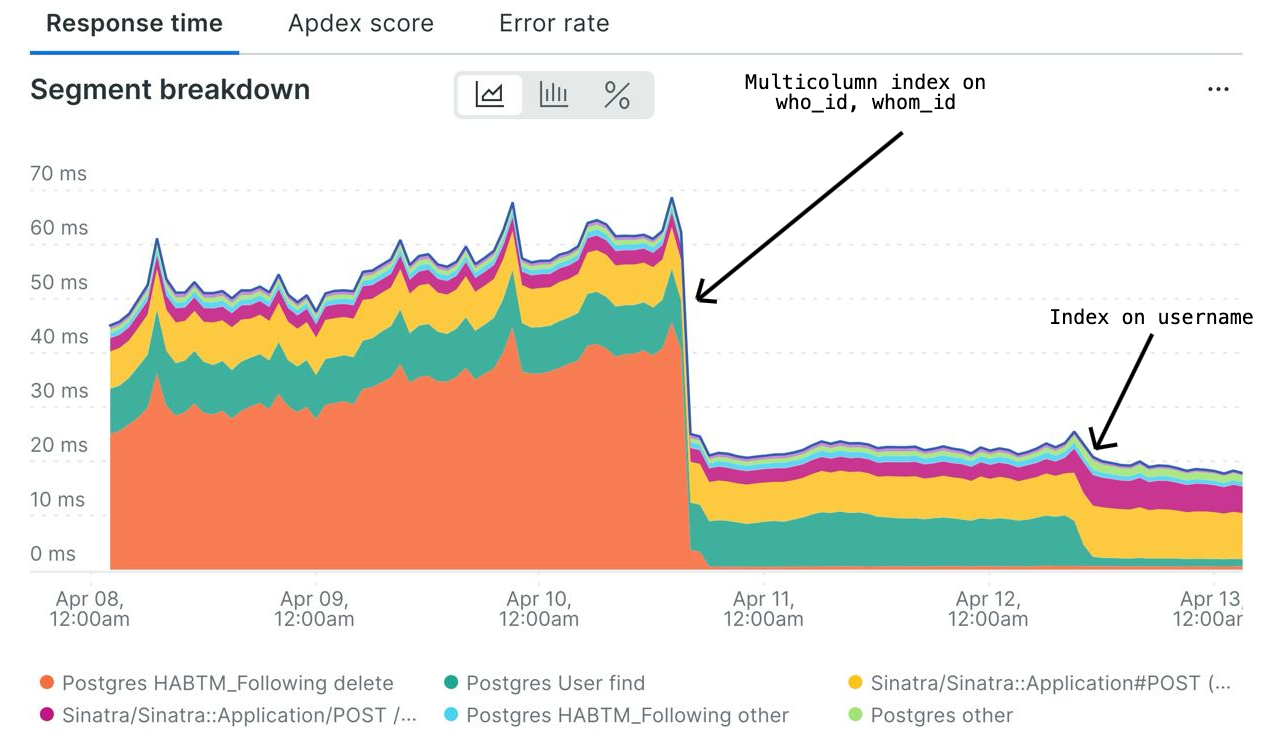
\includegraphics[width=\textwidth]{images/index_apm.png}
    \caption{The APM graph on new relic, before and after adding indexes}
    \label{fig:index_apm}
\end{figure}
\\Similarly, looking at the graph we saw that a considerable amount of time was spent on the \texttt{GET /user} endpoint. Since users are found by querying by the username, we realized this could be fixed with an index on username. The effect of this can be seen on Figure \ref{fig:index_apm}.
% using a managed product for a database was also a learning and a new way of working in this project (less stuff to manage)




\paragraph{Continous deployment}
% Name open for change
% GitOps tool to avoid discrepancies in /remote_files
% Hot fix to avoid downtime and then fix code smells later (weave in different from other projects with DoDs)
% (weave in with testing in CI and such)
When deploying using our deployment pipeline, we would be using some files that are located in \texttt{./remote\_files/}, responsible for pulling the Docker images and starting the Docker swarm. These files are usually uploaded to the manager node using Vagrant or manually \texttt{scp}'ing the files onto the machine. This allows the Github Actions workflow to execute the \texttt{./remote\_files/deploy.sh} script.
However, since we don't often make changes to these files, we would risk forgetting to upload these files when we would actually make changes and there would be room for error causing unwanted or unexpected behaviour.
This caused an issue for us, for example when we had to migrate our database\footnote{\href{https://github.com/git-gurus-itu-devops/itu-minitwit/issues/25\#issuecomment-1983695933}{https://github.com/git-gurus-itu-devops/itu-minitwit/issues/25\#issuecomment-1983695933}}. This margin for error could be decreased by using a declarative language to configure our infrastructure such as Ansible\footnote{\href{https://www.ansible.com/}{https://www.ansible.com/}}, or a simpler imperative solution by copying over the files in the deployment workflow.
% evt. noget om testing i CI men i am not sure hvilken vinkel



\subsection{Evolution and refactoring}


% Our ffirst major downtime came in the form of migrating our SQLITE dartabase to a managed postgersql database. We created a migration script to insert the adat from yhe sqlite db to our postgres db, but this created issues when we ran it. The first issue was the massive amount of data we were trying to insert; we overestimated how much postgres would be able to handle so it died after a while and rolled back the changes. We fixed this by performing the insertions in batches of 1000 instead of trying to perform them all, this allowed to migration to work. The second issue was how regarding primary keys, in that we forgot to also copy the SEQUENCES from the sqlite db, so the new database did not understand how to number the new records, creating duplicate entries. This we fixed by manually restting the sequences to the expected keys. The third issue was in deploying the new deploy script, which we had issues with because Vagrant managed the files on the remote machine. To sync them we would then need to run "vagrant up" but this would also cause downtime. We then manually SCP'ed over the changes.
% An important lesson here is in how to deploy changes to infrastructure, as we did not have an idempotent way of doing this, resulting in having to manually copy over of restart thedroplet. Being able to sync changes in deploy scripts or infrastructure configurations using a GitOps tool would be ver nice.


\subsection{Operation}
% Når man har mulighed for at bruge noget der er managed så gør det. Hold kæft hvor er det nemt.
% Hvis kunne have sparet så meget tid på at bruge managed DigitalOcean load balancing (men måske noget med omkostninger, hvem ved - det er ikke mig der betaler)

\newpage
\printbibliography[
heading=bibintoc
]

\newpage
\section{Appendix}

\subsection{Development dependency graph} \label{appendix: dev-dependecies}
\begin{figure}[H]
    \centering
    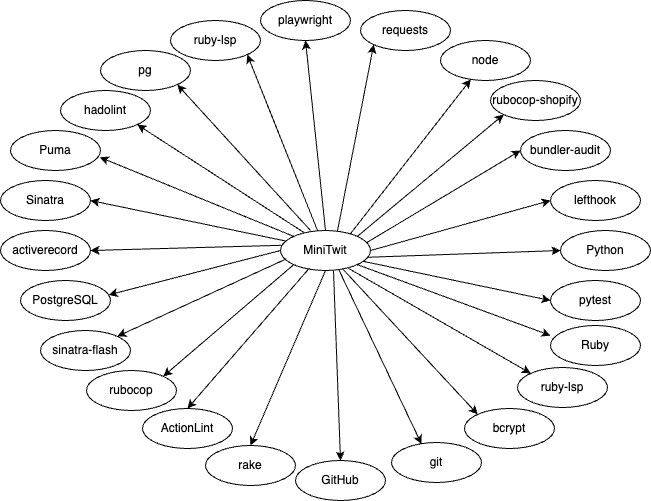
\includegraphics[width=\textwidth]{images/dependency-graph-dev.png}
    \caption{Development dependency graph.}
    \label{fig:dep-dev}
\end{figure}

\end{document}





